%----------------------------------------------------------------------------------------
%	PAQUETES Y OTRAS COSAS DE CONFIGURACION
%----------------------------------------------------------------------------------------
%\documentclass[a4paper,man,natbib,scrbook]{apa6}
\documentclass[12pt]{article}

% esto es una prueba de comment
\usepackage[spanish]{babel}
\usepackage[utf8x]{inputenc}
\usepackage{graphicx}
%\usepackage[colorinlistoftodos]{todonotes} %PAQUETE QUE FALLA JULIO
\usepackage[bottom]{footmisc}
%\usepackage{blindtext} %PAQUETE QUE FALLA JULIO
\usepackage{caption}
\graphicspath{ {images/} }
%\graphicspath{{/home/cursoredes/images/}}
\usepackage{fancyhdr}
\usepackage{enumitem}
\usepackage{hyperref} %INDICE CON VINCULOS
\usepackage{csquotes}

%----------------------------------------------------------------------------------------
%	PAGE HEADERS
%----------------------------------------------------------------------------------------
\setlength{\headheight}{15pt}

\pagestyle{fancy}
\renewcommand{\sectionmark}[1]{ \markright{#1} }

% L=left, R=right, E=even, O=odd

\fancyhf{}
\fancyhead[LE,RO]{\thepage} %Numero pagina
\fancyhead[RE]{\textit{ \nouppercase{\leftmark}} }
\fancyhead[LO]{\textit{ \nouppercase{\rightmark}} }

\fancypagestyle{plain}{ 
  \fancyhf{} 
  \renewcommand{\headrulewidth}{0pt} 
  \renewcommand{\footrulewidth}{0pt}
}
%------------------------------------------------
%
%------------------------------------------------

\begin{document}

\begin{titlepage}

\newcommand{\HRule}{\rule{\linewidth}{0.5mm}} 

\center % Centra todo
 
 
%----------------------------------------------------------------------------------------
%	LOGO SECCION
%----------------------------------------------------------------------------------------

\textsc{\LARGE Universidad Complutense de Madrid}\\[0.1cm] % Universidad

\begin{center}
	\centering
	
\includegraphics[width=0.5\textwidth]{logo}
\end{center}
 
 
%----------------------------------------------------------------------------------------
%	HEADING SECCION
%----------------------------------------------------------------------------------------

\textsc{\LARGE Grupo 4}\\[0.1cm] % Grupo
%\textsc{\Large Heading 1}\\[0.5cm] % Heading mayor
%\textsc{\large Heading 2}\\[0.5cm] % Heading menor

%\textsc{\LARGE Grupo 4}\\[1cm]

%----------------------------------------------------------------------------------------
%	TITULO SECCION
%----------------------------------------------------------------------------------------

\HRule \\[0.4cm]
{ \huge \bfseries HITO 3: FRAMEWORK DE DISEÑO }\\[0.4cm] % Titulo
{ \huge \bfseries MODELADO Y REQUISITOS}\\[0.2cm] % Titulo
\HRule \\[1.2cm]
 
%----------------------------------------------------------------------------------------
%	AUTHOR SECTION
%----------------------------------------------------------------------------------------

\begin{minipage}{0.4\textwidth}
\begin{flushleft} \large
\emph{Autores:}\\
Ángel \textsc{Cruz} \\ %Nombres
Julio \textsc{de la Cruz} \\
Eduardo \textsc{Alcober}\\
Sergio \textsc{Gómez}\\
Isauro \textsc{López}\\
Darío \textsc{Gallegos}
\end{flushleft}
\end{minipage}
\begin{minipage}{0.4\textwidth}
\begin{flushright} \large
\emph{Profesor:} \\
Antonio \textsc{Sánchez} % NOMBRE PROFESOR
\end{flushright}
\end{minipage}\\[0.85cm]
%----------------------------------------------------------------------------------------
%	FECHA SECCION
%----------------------------------------------------------------------------------------
{\large 11 de noviembre de 2018}\\[0.5cm] % Fecha

%---------------------------------------------------------------------------------------
%	CONTENIDO
%----------------------------------------------------------------------------------------

\vfill % Rellenar el resto con espacio en blanco

\end{titlepage}


%\maketitle
%\footnotetext{EJEMPLO DE NOTA A PIE DE PAGINA}

\tableofcontents % Indice de contenidos
\newpage

%----------------------------------------------------------------------------------------
%	INTRODUCCION
%----------------------------------------------------------------------------------------

\section{Introducción}





\section{Alcance del hito}
Se ha de explicar porque nos vamos a centrar en el usuario y no en el resto de roles, como va ha afectar a la aplicación.


\section{Organización y reparto de tareas}
\begin{itemize}

\item \textbf{Documentación}: Permite a todos los miembros de nuestro grupo disponer de las aptitudes y conocimientos necesarios para el siguiente hito.

\item \textbf{Correcciones del hito anterior}: Tras recibir el feedback del anterior hito, es
necesario aplicar las correcciones en general para la entrega final.

\item \textbf{Diseño de un boceto conceptual}:

\item \textbf{Escenarios keypath}:

\item \textbf{Escenarios de vaidación}: 

\item \textbf{Documento de elementos}:

\item \textbf{Mockups de la aplicación}:

\item \textbf{Un diseño final}: 

\begin{center}
	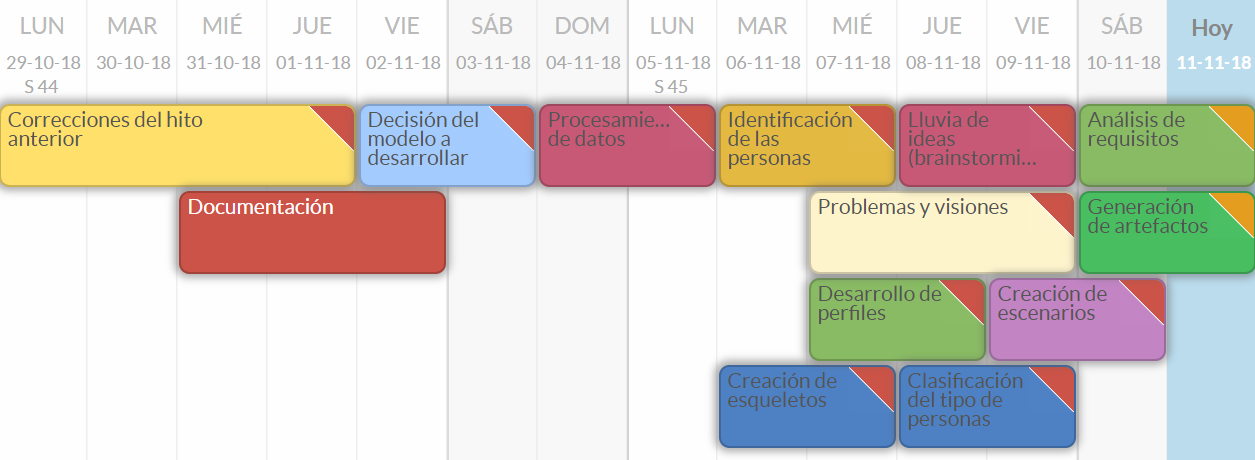
\includegraphics[width=1\textwidth]{planificacionHito2.png}
		\captionof{figure}{Planificación de tareas \href{https://drive.google.com/open?id=1QrF7eOGcyh01kO7jcbpZVWYKA_dWRhWB}{(PDF: planificacionHito2.pdf)} }
\end{center}
\phantom{10}

Los miembros del grupo trabajaremos con un esquema descentralizado controlado, donde las tareas asignadas a cada miembro podrán ser intercambiadas hacia otro; contemplando alguna incidencia si fuera el caso. Luego los miembros del grupo repasamos en profundidad todos los documentos a entregar.

\end{itemize}
\newpage

%----------------------------------------------------------------------------------------
%	DEFINIR LOS PUNTOS DE VISTA QUE USAMOS PARA GENERAR EL PROTOTIPO
%----------------------------------------------------------------------------------------

\section{Definiciones del  framework  de iteracción}
Nota : Modificar la introduccion, hay que hacer enfasesis en que nos vamos a centrar en la interfaz del alumno

Apoyándonos en Sinnaps, una aplicación para la gestión de proyectos, de la misma manera que utilizamos en el hito 1, hemos querido distribuir el reparto de tareas con el objetivo de completar este hito que forma parte de nuestro proyecto final. Las tareas contienen los aspectos más importantes a cumplir, siendo las mismas divididas en subtareas. Detallamos las siguientes con el orden de prioridad correspondiente:

\subsection{Definición del factor de forma}
\subsection{Definición de la postura}
\subsection{Definicion del método de entrada}
\subsection{Definición de los elementos de datos y funcionales }
    \subsubsection{Elementos de datos}
    \subsubsection{Elementos funcionales}


\newpage
%----------------------------------------------------------------------------------------
%	BOCETOS DEL FRAMEWORK DE ITERACCIÓN
%----------------------------------------------------------------------------------------
\section{Bocetos del framework de iteracción}

UNA INTRODUCCION\\

PONER EL ESQUEMA/ESQUELETO DE LA APLICACIÓN Y EXPICARLO\\

CONTINUACIÓN PONER UNOS  BOCETOS MUY SENCILLOS (mockaup de baslamyq) PARA MOSTRAR MUY POR ENCIMA EL FUNCIONAMIENTO DE LA APLICACION.\\


\newpage
%--------------------------------------------------------------------------------------------
%   ESCENARIOS KEYPATH
%--------------------------------------------------------------------------------------------
\section{Escenarios keypath}

Partiendo de los escenarios del hito anterior, narramos el proceso de uso de la aplicación para caso. Por ejemplo, Alex quiere reservar una mesa para estudiar. Enciende su movil y accede a la aplicación. Al ser la primera vez que la usa, debe introducir su cuenta de ucm y contraseñas. Las proximas veces que entre no será necesario. Pulsa en el boton de enter y va a la pagina princial. En el meú inferior pulsa el item puesto libre el cual ...

%--------------------------------------------------------------------------------------------
%   VALIDACIÓN DE LOS DISEÑOS
%--------------------------------------------------------------------------------------------
\section{Validación de los diseños}

%--------------------------------------------------------------------------------------------
%   PROCESO ITERATIVO
%--------------------------------------------------------------------------------------------
\section{Proceso iterativo}

%--------------------------------------------------------------------------------------------
%   CONCLUSIONES
%--------------------------------------------------------------------------------------------
\section{Conclusiones}

\end{document}

%COMENTAARIOS
% \todo[inline, color=green!40]{EJEMPLO DE COMENTARIO}

% PARA INCLUIR UNA FOTOGRAFIA:
%\begin{figure}
%\centering
%\includegraphics[width=0.5\textwidth]{~/DIRECCION/A/IMAGEN.jpg}
%\caption{\label{fig:imagen}DESCRIPCION.}
%\end{figure}

% \dots

% ENUMERACION:
%\begin{enumerate}
%\item Enumeracion 1
%\item Enumeracion 2
%\end{enumerate}

%\begin{itemize}
%\item PUNTO 1

% PARA INCLUIR UNA TABLA:
%\begin{table}[h] %LA h PARA INDICAR QUE LA TABLA NO SEA FLOATING
%\centering
%\begin{tabular}{l|r}
%Fila 0 \\\hline
%Fila 1 & Contenido 1 \\
%Fila 2 & Contenido 2
%\end{tabular}
%\caption{\label{tab:widgets}Ejemplo de tabla.}
%\end{table}

%\item PUNTO 2
%\end{itemize}

%\bibliography{BIBLIOGRAFIA}


